\documentclass[12pt]{article}
\usepackage[utf8]{inputenc}
\usepackage{booktabs}
\usepackage{geometry}
\usepackage{graphicx}
\geometry{a4paper, margin=1in}
\title{Results of the Fisher Combined Test}
\author{Sara Fraija}
\date{\today}
\begin{document}
\maketitle
\section{Resultados}

\begin{table}[h!]
\centering
\resizebox{\textwidth}{!}{%
\begin{tabular}{l c c c c c c}
\toprule
\textbf{GRB} & \textbf{Transit} & \textbf{Significance} & \textbf{Significance Corregida} & \textbf{p-value} & \textbf{Corrected p-value} & \textbf{PDF} \\ \midrule
GRB170708046 & 1 & 0.00 & -3.32 & 5.000e-01 & 9.995e-01 & 6.011e-01 \\
GRB170816599 & 1 & 1.69 & 0.24 & 9.545e-01 & 4.040e-01 & 9.043e-01 \\
GRB170403583 & 1 & 0.00 & -5.01 & 5.000e-01 & 1.000e+00 & 6.011e-01 \\
GRB170826369 & 1 & 0.43 & -4.63 & 6.664e-01 & 1.000e+00 & 6.363e-01 \\
GRB190515190 & 1 & 0.00 & -6.71 & 5.000e-01 & 1.000e+00 & 6.011e-01 \\
GRB230512269 & 1 & 0.76 & -0.35 & 7.764e-01 & 6.367e-01 & 7.011e-01 \\
GRB150101641 & 1 & 1.21 & 1.21 & 8.869e-01 & 1.131e-01 & 8.081e-01 \\
GRB150110923 & 1 & 0.98 & 0.98 & 8.365e-01 & 1.635e-01 & 7.532e-01 \\
GRB150120123 & 1 & 1.86 & 1.86 & 9.686e-01 & 3.144e-02 & 9.293e-01 \\
GRB151229285 & 1 & 0.27 & 0.27 & 6.064e-01 & 3.936e-01 & 6.153e-01 \\
GRB160612842 & 1 & 0.00 & -0.00 & 5.000e-01 & 5.000e-01 & 6.011e-01 \\
GRB160624477 & 1 & 0.76 & 0.76 & 7.764e-01 & 2.236e-01 & 7.011e-01 \\
GRB160821937 & 1 & 1.04 & 1.04 & 8.508e-01 & 1.492e-01 & 7.677e-01 \\
GRB170318644 & 1 & 0.00 & -0.00 & 5.000e-01 & 5.000e-01 & 6.011e-01 \\
GRB170803729 & 1 & 0.00 & -0.00 & 5.000e-01 & 5.000e-01 & 6.011e-01 \\
GRB170817529 & 1 & 2.53 & 2.53 & 9.943e-01 & 5.703e-03 & 9.837e-01 \\
GRB180204109 & 1 & 1.67 & 1.67 & 9.525e-01 & 4.746e-02 & 9.011e-01 \\
GRB180418281 & 1 & 1.04 & 1.04 & 8.508e-01 & 1.492e-01 & 7.677e-01 \\
GRB180715755 & 1 & 0.83 & 0.83 & 7.967e-01 & 2.033e-01 & 7.173e-01 \\
GRB180718082 & 1 & 0.71 & 0.71 & 7.611e-01 & 2.389e-01 & 6.899e-01 \\
GRB180805543 & 1 & 0.00 & -0.00 & 5.000e-01 & 5.000e-01 & 6.011e-01 \\
GRB181125371 & 1 & 0.00 & -0.00 & 5.000e-01 & 5.000e-01 & 6.011e-01 \\
GRB190427190 & 1 & 2.59 & 2.59 & 9.952e-01 & 4.799e-03 & 9.861e-01 \\
GRB201008443 & 1 & 1.54 & 1.54 & 9.382e-01 & 6.178e-02 & 8.781e-01 \\
GRB201214672 & 1 & 2.85 & 2.85 & 9.978e-01 & 2.186e-03 & 9.931e-01 \\
GRB210323918 & 1 & 1.03 & 1.03 & 8.485e-01 & 1.515e-01 & 7.653e-01 \\
GRB210827416 & 1 & 0.00 & -0.00 & 5.000e-01 & 5.000e-01 & 6.011e-01 \\
GRB211024065 & 1 & 0.00 & -0.00 & 5.000e-01 & 5.000e-01 & 6.011e-01 \\
GRB220412713 & 1 & 0.63 & 0.63 & 7.357e-01 & 2.643e-01 & 6.729e-01 \\
GRB220418720 & 1 & 0.53 & 0.53 & 7.019e-01 & 2.981e-01 & 6.533e-01 \\
GRB220511571 & 1 & 0.45 & 0.45 & 6.736e-01 & 3.264e-01 & 6.395e-01 \\
GRB220617772 & 1 & 0.00 & -0.00 & 5.000e-01 & 5.000e-01 & 6.011e-01 \\
GRB221120895 & 1 & 0.00 & -0.00 & 5.000e-01 & 5.000e-01 & 6.011e-01 \\
GRB230228244 & 1 & 0.00 & -0.00 & 5.000e-01 & 5.000e-01 & 6.011e-01 \\
GRB230812790 & 1 & 0.09 & 0.09 & 5.359e-01 & 4.641e-01 & 6.027e-01 \\
GRB170708046 & 2 & 0.27 & -2.66 & 6.064e-01 & 9.961e-01 & 6.153e-01 \\
GRB170816599 & 2 & 1.31 & -0.44 & 9.049e-01 & 6.705e-01 & 8.309e-01 \\
GRB170206453 & 2 & 0.00 & -6.24 & 5.000e-01 & 1.000e+00 & 6.011e-01 \\
GRB170403583 & 2 & 1.64 & -0.46 & 9.495e-01 & 6.765e-01 & 8.960e-01 \\
GRB170826369 & 2 & 3.03 & 1.76 & 9.988e-01 & 3.906e-02 & 9.960e-01 \\
GRB190515190 & 2 & 1.06 & -2.71 & 8.554e-01 & 9.967e-01 & 7.725e-01 \\
GRB200605762 & 2 & 0.90 & -1.77 & 8.159e-01 & 9.614e-01 & 7.339e-01 \\
GRB230512269 & 2 & 0.00 & -1.53 & 5.000e-01 & 9.375e-01 & 6.011e-01 \\
GRB150101641 & 2 & 0.25 & 0.25 & 5.987e-01 & 4.013e-01 & 6.133e-01 \\
GRB150110923 & 2 & 1.81 & 1.81 & 9.649e-01 & 3.515e-02 & 9.225e-01 \\
GRB151229285 & 2 & 1.01 & 1.01 & 8.438e-01 & 1.562e-01 & 7.604e-01 \\
GRB160624477 & 2 & 1.73 & 1.73 & 9.582e-01 & 4.182e-02 & 9.107e-01 \\
GRB160714097 & 2 & 0.00 & -0.00 & 5.000e-01 & 5.000e-01 & 6.011e-01 \\
GRB170318644 & 2 & 0.27 & 0.27 & 6.064e-01 & 3.936e-01 & 6.153e-01 \\
GRB170803729 & 2 & 0.25 & 0.25 & 5.987e-01 & 4.013e-01 & 6.133e-01 \\
GRB170817529 & 2 & 1.58 & 1.58 & 9.429e-01 & 5.705e-02 & 8.855e-01 \\
GRB171007498 & 2 & 0.00 & -0.00 & 5.000e-01 & 5.000e-01 & 6.011e-01 \\
GRB180204109 & 2 & 0.84 & 0.84 & 7.995e-01 & 2.005e-01 & 7.197e-01 \\
GRB180402406 & 2 & 0.16 & 0.16 & 5.636e-01 & 4.364e-01 & 6.061e-01 \\
GRB180418281 & 2 & 1.28 & 1.28 & 8.997e-01 & 1.003e-01 & 8.242e-01 \\
GRB180715755 & 2 & 0.46 & 0.46 & 6.772e-01 & 3.228e-01 & 6.411e-01 \\
GRB180718082 & 2 & 2.76 & 2.76 & 9.971e-01 & 2.890e-03 & 9.912e-01 \\
GRB180805543 & 2 & 0.72 & 0.72 & 7.642e-01 & 2.358e-01 & 6.921e-01 \\
GRB181125371 & 2 & 0.87 & 0.87 & 8.078e-01 & 1.922e-01 & 7.268e-01 \\
GRB190427190 & 2 & 0.00 & -0.00 & 5.000e-01 & 5.000e-01 & 6.011e-01 \\
GRB200623138 & 2 & 0.00 & -0.00 & 5.000e-01 & 5.000e-01 & 6.011e-01 \\
GRB201008443 & 2 & 0.00 & -0.00 & 5.000e-01 & 5.000e-01 & 6.011e-01 \\
GRB201214672 & 2 & 2.11 & 2.11 & 9.826e-01 & 1.743e-02 & 9.569e-01 \\
GRB210323918 & 2 & 0.00 & -0.00 & 5.000e-01 & 5.000e-01 & 6.011e-01 \\
GRB210618072 & 2 & 1.19 & 1.19 & 8.830e-01 & 1.170e-01 & 8.035e-01 \\
GRB210827416 & 2 & 0.00 & -0.00 & 5.000e-01 & 5.000e-01 & 6.011e-01 \\
GRB220412713 & 2 & 1.29 & 1.29 & 9.015e-01 & 9.853e-02 & 8.264e-01 \\
GRB220418720 & 2 & 2.11 & 2.11 & 9.826e-01 & 1.743e-02 & 9.569e-01 \\
GRB220511571 & 2 & 1.45 & 1.45 & 9.265e-01 & 7.353e-02 & 8.606e-01 \\
GRB220617772 & 2 & 1.78 & 1.78 & 9.625e-01 & 3.754e-02 & 9.182e-01 \\
GRB221120895 & 2 & 0.00 & -0.00 & 5.000e-01 & 5.000e-01 & 6.011e-01 \\
GRB230228244 & 2 & 0.00 & -0.00 & 5.000e-01 & 5.000e-01 & 6.011e-01 \\
GRB230812790 & 2 & 0.92 & 0.92 & 8.212e-01 & 1.788e-01 & 7.387e-01 \\
\bottomrule
\end{tabular}%
}
\caption{Lista de GRBs with sus Transits, Significances, Significances Corregidas, p-values, p-values Corregidos y valores PDF.}
\end{table}

\begin{figure}[h!]
\centering
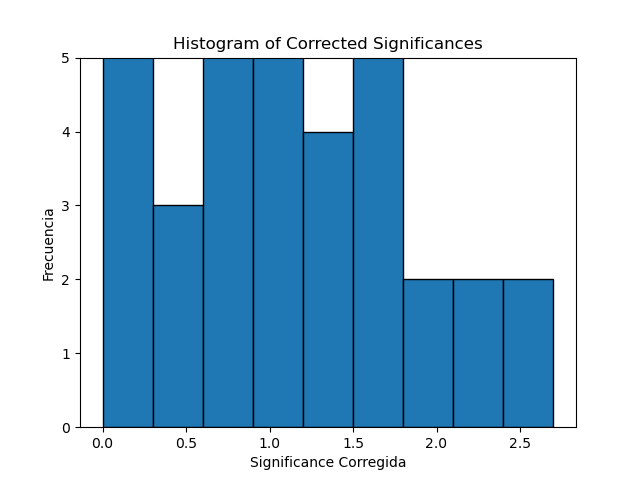
\includegraphics[width=0.6\textwidth]{corrected_significance_hist.png}
\caption{Histogram of Corrected Significances.}
\end{figure}

\section*{Conclusion}
The Fisher combined test integrates individual p-values to evaluate a global hypothesis.
The resulting test statistic was $X^2 = 226.294$ with 146 degrees of freedom.
For a significance level of 0.05, the critical value is 175.198.
Since $X^2$ is greater than the critical value, we rechazamos the null hypothesis of independence.
Normal approximation: p-value = 2.345e-05, significance ≈ 4.07 sigma.

\end{document}